%% Lee
%% In dissertation, change 
%    section* to chapter 
%    subsection* to section
%    subsubsection* to subsection


% #######################################################################################################################################
\chapter{Detailed System Description}
\label{chap-five}
%\label{sec:detailedSystemDescription}

A detailed flow diagram and block diagram of the sub-system column can be seen in figures \ref{fig:DetailedFlowDiagram} and \ref{fig:DetailedBlockDiagram} respectively.
\begin{figure}
% the [] contains position info e.g. [!t] means here
\centering
\captionsetup{justification=centering}
\captionsetup{width=.9\linewidth}
\centerline{
\mbox{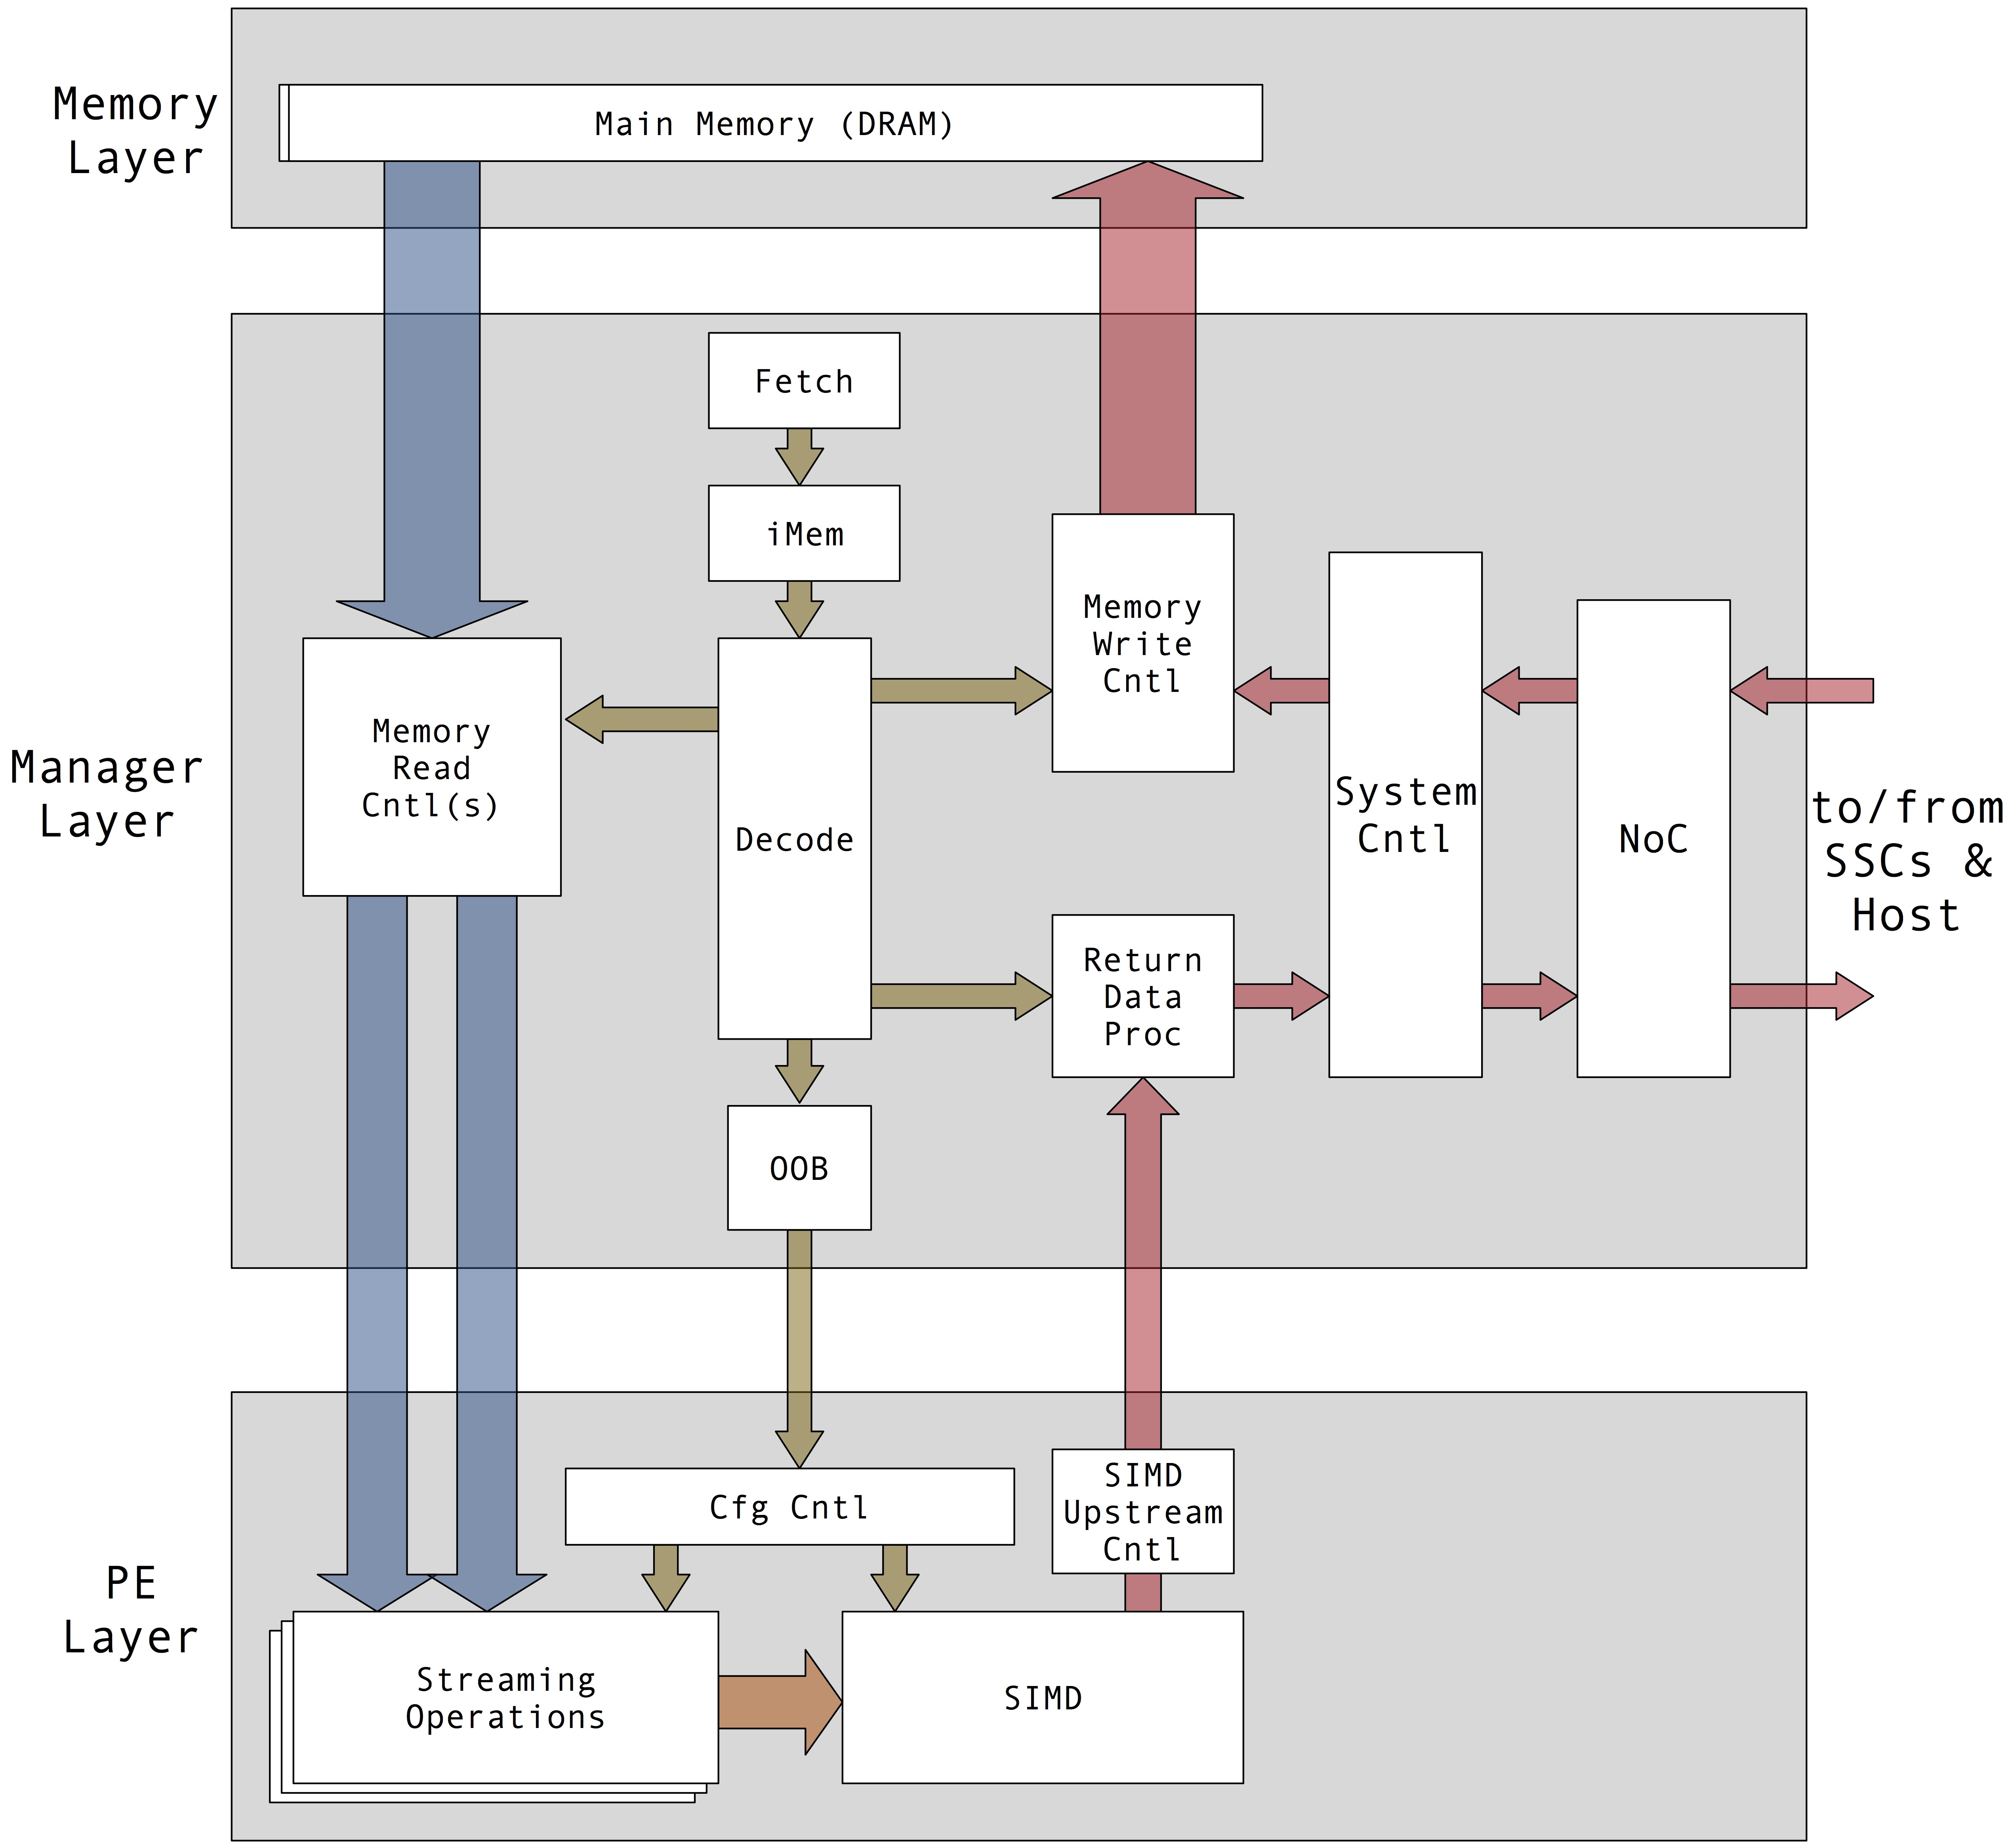
\includegraphics[scale=0.07]{DetailedFlowDiagram.jpg}}
}
\center\caption{Sub-System Column (SSC) Detailed Flow Diagram}
\label{fig:DetailedFlowDiagram}
\end{figure}

\begin{figure}[t]
% the [] contains position info e.g. [!H] means here
% H 	Place exactly at spot in source text
% h 	Place approximately at spot in source test
% t 	Place at top of page
% b 	Place at bottom of page
% p 	Place on page for floats only
% ! 	Override internal LaTeX parameters for determining float position
\centering
\captionsetup{justification=centering}
\captionsetup{width=.9\linewidth}
\centerline{
\mbox{
\includegraphics[angle=90, height=8in]{DetailedBlockDiagram.jpg}}
}
\center\caption{Sub-System Column (SSC) Detailed Block Diagram}
\label{fig:DetailedBlockDiagram}
\end{figure}

\section{Manager}
\label{sec:manager}

\subsection{Operation Decode}
\label{ssec:operationDecode}

In figure \ref{fig:DetailedBlockDiagram}, instructions are read from instruction memory and passed to the instruction decoder.

The operation tuple is decoded and a streaming operation (stOp) pointer and a SIMD operation pointer are sent to the PE inside an OOB control packet.

The stOp pointer specifies what streaming operation is to take place on the data directly streamed to the PE. In the baseline system, typically this would be a floating-point multiply accumulate on two arguments, the pre-synaptic neuron states and the pre-synaptic weights.

The SIMD pointer is essentially a program counter that will be invoked when the stOp result is passed to the SIMD.

Note that other types of stOp includes a NOP with a destination of local memory. This allows us to transfer block of instruction or data from the manager to the PE.


\subsection{Argument Decode}
\label{ssec:argumentDecode}
The instruction also includes argument descriptors. These descriptors include a storage descriptor pointers that point to a storage descriptor stored in local memory that encodes where data should be read from for the one or two arguments that will be streamed from DRAM to the stOp within the PE. In the case of a AN activation calculation, there are two arguments, the pre-synaptic neuron states and the pre-synaptic weights. The read storage descriptor pointers are passed to the Memory Read Controllers (MRC). The MRCs read the actual storage descriptor from their local memory and immediately start sending read commands to the memory via a Main Memory Controller (MMC). The MMC is not shown in the diagram but essentially takes the memory read requests and converts them into the DRAM read protocol.

As soon as read data is sent back to the MRC via the MMC, that data is aligned with the downstream bus and sent to the 32 Streaming Operations inside the PE.


\subsection{Result data Processing}
\label{ssec:resultDataprocessing}
The instruction also includes argument descriptors. These descriptors include a storage descriptor pointers that point to a storage descriptor stored in local memory that encodes where data should be read from for the one or two arguments that will be streamed from DRAM to the stOp within the PE. In the case of a AN activation calculation, there are two arguments, the pre-synaptic neuron states and the pre-synaptic weights. The read storage descriptor pointers are passed to the Memory Read Controllers (MRC). The MRCs read the actual storage descriptor from their local memory and immediately start sending read commands to the memory via a Main Memory Controller (MMC). The MMC is not shown in the diagram but essentially takes the memory read requests and converts them into the DRAM read protocol.

As soon as read data is sent back to the MRC via the MMC, that data is aligned with the downstream bus and sent to the 32 Streaming Operations inside the PE.


\subsection{Memory Write Controller}
\label{ssec:memoryWriteController}

The Memory Write Controller (MWC) receives data from to sources, the NoC via the MCNTL and the RDP.

In both cases, the MWC read the actual storage descriptor from their local memory and immediately start forming data that will be written back to main memory.

When the data is formed, a write command is sent to the memory via the MMC. Again, the MMC is not shown in the diagram but takes the memory write requests along with the data and converts them into the DRAM write protocol.

The MWC can only operate on one of the two sources at any one time. However, there are four 4096-bit holding registers where data is formed prior to the write request.

The holding registers have the potential in future to allow aggregation of data from one or more operations to allow a coalesced write back to main memory.


\section{Processing Engine}
\label{sec:pe}

\subsection{Configuration}
\label{ssec:peConfiguration}

A configuration controller within the PE (PE\_CNTL) takes the OOB packet from the Manager and extracts the stOp and SIMD operation pointers.

The stOp pointer is used to point to a local stOp configuration memory. The memory contains the various configuration data required by the streaming operation controller (stOp\_CNTL). The stOp\_CNTL is not shown.

The stOp\_CNTL configures the:

\begin{outline}
    \1 Operation type
    \1 Number of active execution lanes
    \1 Source of the argument data, which can be downstream data from the manager or from the small local SRAM
    \1 Destination of the result data, which can be the SIMD or the small local SRAM
\end{outline}

The SIMD operation pointer is sent to the SIMD.

\subsection{Streaming Operations}
\label{ssec:stOps}

The streaming Operations (stOp) are designed to operate on data passed from the Manager at or near line-rate. If line-rate cannot be maintained, a flow-control mechanism is employed to slow the data from the Manager.

Once the stOp has processed the data, it passes the result to the SIMD. Note in some cases the result can be placed in local SRAM or sent to both SIMD and SRAM.

It should also be stated that while the stOp is processing the current data, the SIMD may be operating on the result of the previous operation. It is expected the SIMD will have completed the previous operation before the stOp completes the current operation, but again, if necessary a flow control mechanism between SIMD and stOP will be engaged if the SIMD is not ready.

\subsection{SIMD}
\label{ssec:simd}

The SIMD takes the result data and performs the operation starting at the program counter (PC) indicated by the SIMD operation pointer provided by the PE\_CNTL.

The stOp provides the result to the SIMD via a local register. The result is also written, in most cases to the small local SRAM.

The SIMD performs the specified operation on the data provided by the stOp.

In most cases this will be the AN activation function and in the baseline system is the Rectified Linear function (ReLu).

When the SIMD has completed its operation, it passes the result to the SIMD Upstream controller to be returned to the Manager.

\subsection{Result Data}
\label{ssec:result}

The SIMD Upstream Controller (SUI) takes the data and encapsulates it in an Upstream packet. Included in the packet is the tag required by the Return Data processor within the Manager.



